\documentclass[12pt]{article}
\usepackage{minted}
\usepackage{graphicx}
\usepackage[margin=0.25in]{geometry}

\begin{document} 
	\noindent
	Dan Jandel C. De Ramos\\
	BSCpE 2-1\\
	Made with \LaTeX \\
	\\
	Activity 2 using nextLine()\\
	Source Code:
		
	\begin{minted}[tabsize=5]{java}         
/*
* Written by: Dan Jandel C. De Ramos
* Polytechnic University of the Philippines Biñan
* Bachelor of Science in Computer Engineering 2-1
*/

import java.util.Scanner;
import java.util.InputMismatchException;

public class Activity_2{
	public static void main(String[]args){
		
		Scanner input = new Scanner(System.in);
		
		String name;
		String location;
		short age = 0;
		
		System.out.println();
		
		System.out.println("\u2022 Activity # 2 \u2022 \n");
		System.out.println("What is your name? ");
		name = input.nextLine();
		System.out.println("\nWhat is your age in years? ");        
		while(age==0){            
			try {
				age = input.nextShort();
			} catch (java.util.InputMismatchException e) {            
				System.out.print("\n!!! You have entered an invalid value.");
				System.out.println("Please use whole numbers only !!!");  
				System.out.println("What is your age in years?");
				input.next();          
			}
		}
				
		input.nextLine();
		System.out.println("\nWhere do you live?");
		location = input.nextLine();
		input.close();
		System.out.println("\nYour name is " + name);
		System.out.println("You are " + age + " years old");
		System.out.println("You live in " + location);
		
		System.out.println();
	}
}
	\end{minted}
	\clearpage
	\noindent
	Output:\\
	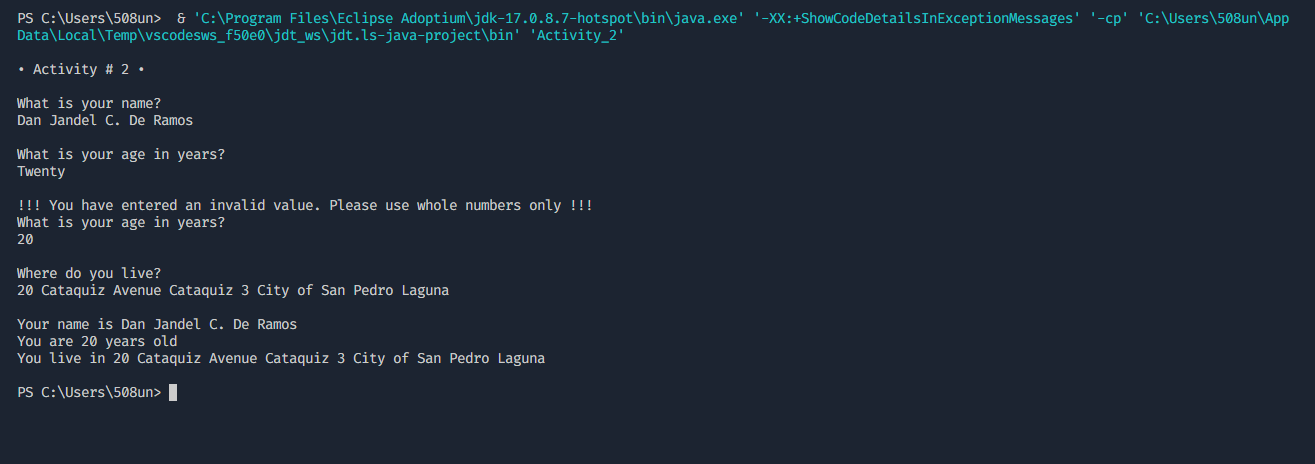
\includegraphics[width=\textwidth]{output}
\end{document}